\chapter{Static Analysis}

\section*{Overview}
\paragraph*{}
Static Analysis has been at the heart of inspecting the behaviour of software, without actually executing it, for decades now. It sits at the core of optimizing compilers, but it also gives room for building external tools such as linters which usually appear in the development pipeline before creating a software release and points developers to the direction of mistakes by printing warnings or errors. Also, automatic error detection is part of most modern Integrated Development Environments \footnote{This is also true for interpreted languages such as R or Python, although detection is not as comprehensive as it is for compiled, statically typed languages} (IDE) such as Visual Studio, Eclipse etc. thanks to static analysis.

\paragraph*{}
There are, of course, some limitations to this technique, a more popular one relating to the Halting problem. As Alan Turing proved in 1936, it is not possible for an algorithm to determine if another will halt for all possible inputs. Anders Møller and Michael I. Schwartzbach best put it in their Static Program Analysis book as follows: \cite[automated reasoning of software generally must involve approximation]{static-program-analysis}. However, this technique can provide \textbf{guarantees} about specific execution paths in a program. The most important aspect here is to not provide false positives, as those could result in optimizing something that should not be optimized or, even worse, change the semantics of a program.

\paragraph*{}
The latter is an ethic similar to the Principle of Least Privilege in Program Security - by default, when doing static analysis, we assume that nothing can be optimized, i.e. worst case possible. As we perform analysis, we build guarantees over what can be optimized by ensuring that specific properties are respected, such as specific flows in the control flow graphs or specific variable states in data flow analysis.

\paragraph*{}
Some examples of what this techniques seeks is:
\begin{itemize}
    \item Are there declared variables that are not used?
    \item Are there assignments for variables that are not referenced anymore after the assignment?
    \item Are there mathematical operations executed that are not referenced and do not change the state of the program?
    \item Are there \textbf{unreachable flows} in the program execution, i.e. dead code?
    \item Are there \lstinline[columns=fixed]{if} conditions that can be computed at compile time? If so, can they be directly replaced with true / false body?
    \item Are there duplicated expressions that can be computed only once? If so, can they be computed at compile time?
\end{itemize}

\paragraph*{}
The above represent common optimization possibilities across programming languages, as well as a small subset of this domain. Depending on the properties of the programming language and the virtual machine that will run the generated bytecode, additional proprietary analysis may be done at compile time.

\paragraph*{}
An example of the benefits of this analysis technique can be seen in two modern Machine Learning technologies, JAX and IREE. These perform computation on tensors, therefore widely used for differentiation operations in neural networks. Since in neural networks the data shape is often known, these technologies can trace the data shapes of the tensors throughout the computation pipeline. This helps with handling memory objects more efficiently, pre-allocating memory buffers, re-using them when necessary and apply parallel computation on memory blocks. This can happen both with Ahead Of Time Compilation (AOT) and Just In Time compilation (JIT), but it of course \cite[requires array shapes to be static \& known at compile time]{jax-to-jit-or-not-to-jit}.

\section{Control Flow Graphs}
\subsection{Overview}
\paragraph*{}
Control Flow Graphs (CFG) are esentially directed graphs $G=(V, E)$, where $V$ is the set of nodes (\textbf{basic blocks}) and $E$ determine the edges (\textbf{control flows}) between the nodes. They act as data structures used to analyse the execution flow in computer programming by following the edges between nodes. That is, it is not necessary for all of the edges to be visited during a program execution, and some nodes can never be visited, regardless of the program input. Since the whole program semantics are embedded into such a graph, we can safely affirm that it represents yet another intermediate representation of a computer program, hence why the operation of CFG generation is \textbf{symmetric} - we can reconstruct a computer program from a CFG.

\paragraph*{}
CFGs are usually applied in situations of \textbf{flow-sensitive analysis} and where the order of the instructions matter. While intermediate representations such as ASTs are syntax-oriented, CFGs are semantic-oriented and can have a significantly difference structure. For example, loops introduce cycles in the CFG, while they do not in an AST.

\begin{figure}
    \centering
    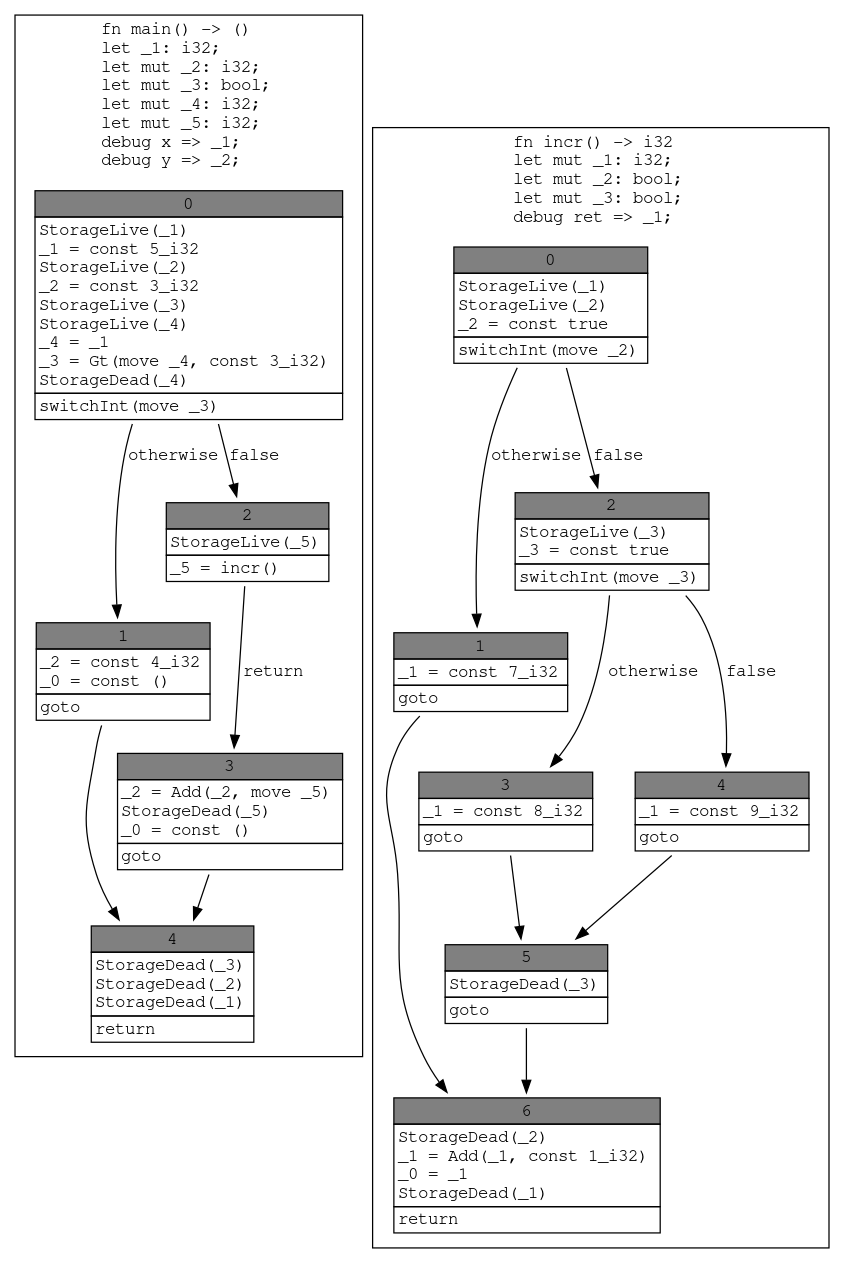
\includegraphics[width=15cm]{images/cfg_rust_example.png}
    \caption{Example of a CFG built on top of a simple Rust program. The entry blocks allocate memory for variables, while the exit block act as garbage collection and terminate the execution flow. Source: Wikipedia}
    \label{fig:cfg-rust-example}
\end{figure}

\subsection{Properties}
\paragraph*{}
We call a graph node $v$ a \textbf{basic block}. The property of a node is that the code instructions it represents are executed sequentially, with no \textbf{interrupting flows} between these. This translates to no \lstinline[columns=fixed]{JUMP} instructions in assembly code. We can easily state that any basic block $v$ containing $n$ instructions can be split into $n$ basic blocks $v_1, v_2, ..., v_n$ since the property of no interrupting flows will be inherited by the ``child nodes''.

\paragraph*{}
The first instruction in such a node is called a \textbf{leader}. Since the transition between nodes is made by jump instructions, the leaders translate to the first assembly instructions after jump instructions. Having observed this, we state that a basic block $i$ starts at leader $L_i$ and ends before leader $L_{i+1}$, property which can be used to generate the basic blocks of a CFG \cite{cfg-dcc}.

\paragraph*{}
Considering a single CPU, the execution of a program means executing assembly operations \textbf{sequentially} on the same processor, hence why a CFG is a directed graph. The edge direction gives us the order of instruction execution, and cycles can be present in this graph (eg. loops). Considering a graph node $v$, we have the following:
$$deg^+(v) \textrm{, the inner degree (indegree) of the node, and}$$
$$deg^-(v) \textrm{, the outer degree (outdegree) of the node.}$$

\paragraph*{}
The inner degree $deg_+(v)$ correspond to all of the possible flows that precede the execution of $v$, so we have
$$deg^+(v) = |\{u, \exists e \in E, e=(u, v), u \in V\}|$$
We call $v$ an \textbf{entry block} if $deg^+(v)=0$, meaning there is no preceding execution flow for $v$, therefore that is the start of the program. Similarly, we call $v$ and \textbf{exit block} if $deg^-(v)=0$, where
$$deg^-(v) = |\{u, \exists e \in E, e=(v, u), u \in V\}|$$
Exit blocks introduce \textbf{termination flows} in the program\footnote{It is possible to have termination flows in basic blocks that have a strictly positive outer degree due to non-jump instructions such as the \lstinline[columns=fixed]{return} command.}.

\subsection{Usage examples. Local and global optimizations}
\paragraph*{}
Code optimizations can be divided based on their context, local or global. Local optimizations are interested in inspecting small blocks of code, abstracting out the surrounding ``environment'' of the code, and these can further build their own representations of basic blocks. Since each instruction within a basic block works with one or more inputs, we can compute a DAG (Directed Acyclic Graph) that tracks input and intermediary variables usage throughout computation. The DAG can further be used to simplify the basic block, such as applying common subexpression elimination, by pruning the DAG wherever possible. The basic block is then rebuilt by walking the DAG and generating the code instructions according to the used dialect.

\paragraph*{}
Another type of local optimization is Peephole optimization, which acts as a shifting window over small portions of a basic block. If basic blocks are granular enough, they can be applied on the whole block directly, however this depends on the CFG generation method. Peephole optimization can be used to apply common subexpression eliminator as well, however it is more concerned in finding specific patterns in the window of focus.

\begin{figure}
    \centering
    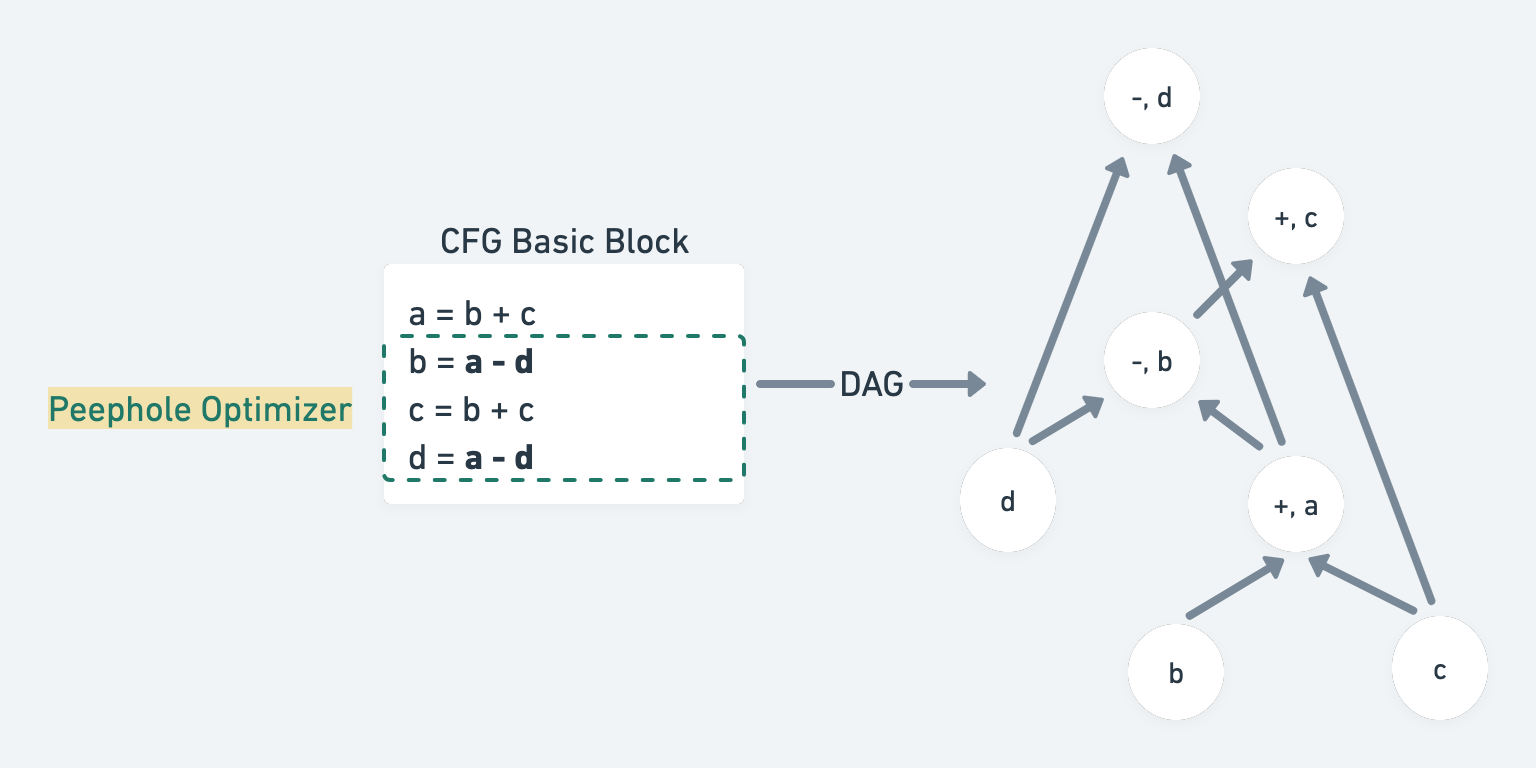
\includegraphics[width=15cm]{images/dag_peephole.png}
    \caption{Representing the inputs of a basic block using DAGs. Example of the peephole optimizer and where common subexpression eliminator could be used.}
    \label{fig:dag-peephole-example}
\end{figure}

\paragraph*{}
Global optimizations \cite[need to analyze the entire control flow graph of a program]{cfg-dcc}, such as figuring out if a computed expression, passed as a parameter through the execution flow is actually ever used. In order to judge such a case, we need to walk multiple paths in a CFG and identify whether there are any basic blocks using the given expression (parameter, variable etc.).

\section{Data Flow Analysis}
\subsection{Overview}
\paragraph*{}
Data flow analysis is one of the dominant techniques of static analysis for reasoning about the flow of data in the program. This expands to the different kinds of data: variables, expressions and constants. It is impossible for a software analysis program to guarantee \textbf{soundness, completeness and termination} at the same time. The compromise that data flow analysis does is to sacrifice completeness, making it \textbf{incomplete}. That is, it will report all facts that could occur during program execution, but also ``false positives'', i.e. facts that will never occur in program runs. The way completeness is sacrificed is by abstracting the control flow conditions, i.e. considering that there is a program run that walks all flow paths, regarding of the control flow conditions (eg. if statement conditions).

\paragraph*{}
Soundness informally means \cite[that the flow functions map abstract information before each instruction to abstract information after that instruction in a way that matches the instruction's concrete semantics]{program-analysis-corectness-cmu}. That is, let's say we have a problem which we represent by a pair of the input and output $P=(I, O)$. We define an abstractization function $DF$ that maps the concrete input $I$ to the abstract domain for the problem $P$:
$$DF(I) = I_a$$
and does the same for the output $O$:
$$DF(O) = O_a$$

\paragraph*{}
In order to have a sound analysis, the data flow analysis must correctly perform modifications to the abstract input $I_a$, according to the correct machine semantics of the program $P$ (eg. x86\_64 ASM instructions) such that after each instruction, a transition function $\sigma$ is applied, such that $S = I_a \rightarrow S = \sigma(S) \rightarrow \cdots \rightarrow S = \sigma(S)$. If the analysis is kept, then $S=O_a$.


% TODO Soundness, completeness and termination.

\begin{lstlisting}[language=Solidity, caption={Simple example of how data flow analysis is used to trace the values of a variable through the execution flow.}]
    // SPDX-License-Identifier: MIT
    pragma solidity ^0.8.14;
    
    contract DataFlowAnalysis {
        uint256 persistent_var;
    
        function variableTracing(uint256 n) public pure returns (uint256) {
            uint256 x; // x is 0
            if (n > 10) {
                x = 1; // x is 1
            } else {
                x = 2; // x is 2
            }
            // x is in {1, 2}
            return x;
        }
    }    
\end{lstlisting}

% \subsection{Examples}
\paragraph*{}
One example is null pointer safety in Dart, which has been very positively received by the developer community as a \cite[boost to productivity]{proxify-dart-null}. Null pointers are often the cause of runtime exceptions, making an application crash without any sign in advance. What null pointer safety does is that it tells the compiler that a variable may or may not be null through the special ``?'' symbol: \lstinline[columns=fixed]{String? hello = "world";}. This way, the compiler can perform data flow analysis and warn the developer in case a null pointer exception might be encountered. It is best put by the Dart documentation itself: \cite[runtime null-dereference errors turn into edit-time analysis errors.]{dart-dev-null-safety}
